\begin{tikzpicture}[xscale=-0.8]
    
    % Define los puntos de un triángulo
    \tkzDefPoint(0,0){A}
    \tkzDefPoint(5,0){B}
    \tkzDefPoint(3,3){C}
    
    % Dibuja el ángulo
    \tkzDrawPolygon(A,B,C)

    %\tkzDrawPoints(A,B,C)
    \tkzLabelPoint[right](A){$D$}
    \tkzLabelPoint[left](B){$E$}
    \tkzLabelPoint[above](C){$F$}
    
    % Dibuja los ángulos marcados
    \tkzMarkAngle[size=1cm](B,A,C)
    %\tkzLabelAngle[pos = 0.7](B,A,C){$\alpha$}
    \tkzMarkAngle[size=1cm](C,B,A)
    \tkzMarkAngle[size=1.1cm](C,B,A)
    %\tkzLabelAngle[pos = 0.7](C,B,A){$\beta$}
    
    % Marca los lados no incluídos con barras
    \tkzMarkSegment[mark=||](A,C)
    
\end{tikzpicture}